\item
\begin{enumerate}
  \item Draw the Bayes net corresponding to this setup.
        \begin{center}
          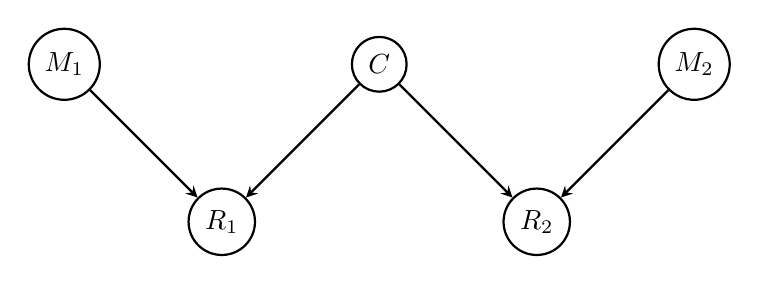
\begin{tikzpicture}[->,>=stealth,auto,node distance=0cm,
              thick,main node/.style={circle,draw}]

            \node[main node] (M1) at (0,2) {$M_1$};
            \node[main node] (R1) at (2,0) {$R_1$};
            \node[main node] (C) at (4,2) {$C$};
            \node[main node] (R2) at (6,0) {$R_2$};
            \node[main node] (M2) at (8,2) {$M_2$};

            \path[every node/.style={}]
            (M1) edge (R1)
            (C) edge (R1)
            (C) edge (R2)
            (M2) edge (R2);

          \end{tikzpicture}
        \end{center}
        \begin{center}
          \bgroup
          \def\arraystretch{1.5}%
          \begin{tabular}{|c|c|p{6cm}|}
            \hline
            Variable Name & Domain        & Interpretation                                                               \\
            \hline
            $C$           & $\{1, 0\}$    & The actual health of a person. Either COVID positive $1$ or negative $0$.    \\
            \hline
            $M_1$         & $\{a, b, c\}$ & The manufacturer of the first test kit. Where the company is $a, b$ or $c$.  \\
            \hline
            $M_2$         & $\{a, b, c\}$ & The manufacturer of the second test kit. Where the company is $a, b$ or $c$. \\
            \hline
            $R_1$         & $\{1, 0\}$    & The result of the first test kit. Either positive $1$ or negative $0$.       \\
            \hline
            $R_2$         & $\{1, 0\}$    & The result of the second test kit. Either positive $1$ or negative $0$.      \\
            \hline
          \end{tabular}
          \egroup
        \end{center}
        This table can be interpreted as three independent events $M_1$, $M_2$ and $C$. The manufacturer of the two test kits received by a person and their actual health are independent, but they will determine the result of the test kit.
  \item Write conditional probabilities (numerical values) associated with each node of this Bayes net. As there are 5 variables, please specify one conditional probability table (CPT) for each variable.
        \begin{center}
          \bgroup
          \def\arraystretch{1.5}%
          \begin{tabular}{|c|c|c|}
            \hline
            $P(C=0)$ & $P(C=1)$ \\
            \hline
            $0.7$    & $0.3$    \\
            \hline
          \end{tabular}
          \egroup
        \end{center}
        \begin{center}
          \begin{center}
            \bgroup
            \def\arraystretch{1.5}%
            \begin{tabular}{|c|c|c|}
              \hline
              $P(M_n=a)$ & $P(M_n=b)$ & $P(M_n=c)$ \\
              \hline
              $0.333$    & $0.333$    & $0.333$    \\
              \hline
            \end{tabular}
            \egroup
          \end{center}
          \bgroup
          \def\arraystretch{1.5}%
          \begin{tabular}{|cc|c|c|}
            \hline
            $M_n$ & $C$ & $P(R_n=0\mid M_n, C)$ & $P(R_n=1\mid M_n, C)$ \\
            \hline
            $a$   & $0$ & $0.99$                & $0.01$                \\
            \hline
            $b$   & $0$ & $0.95$                & $0.05$                \\
            \hline
            $c$   & $0$ & $0.91$                & $0.09$                \\
            \hline
            $a$   & $1$ & $0.3$                 & $0.7$                 \\
            \hline
            $b$   & $1$ & $0.2$                 & $0.8$                 \\
            \hline
            $c$   & $1$ & $0.1$                 & $0.9$                 \\
            \hline
          \end{tabular}
          \egroup
        \end{center}
        For values of $n \in \{1, 2\}$ as each person has two test kits.
  \item Are the results of the two tests dependent or independent given the evidence that the Covid Status is known? Justify your answer.\\[5pt]
        There is a common cause structure $R_1 \leftarrow C \rightarrow R_2$ which couples $R_1$ and $R_2$. But given the COVID status $C$, it decouples $R_1$ and $R_2$. Thus they are independent.
  \item Assume you took both tests at home. After being tested twice in a matter of minutes, the first test was positive and the second negative. What is the probability that you actually have COVID19? Show your analytical computations.\\[5pt]
        Given that the first test was positive and the second test was negative, then
        \begin{align*}
          R_1 & =1 \\
          R_2 & =0
        \end{align*}
        We are trying to solve for $P(C=1\mid R_1=1, R_2=0)$. Since $R_1$ and $R_2$ are conditionally independent on $C$,
        \begin{align*}
          P(C=1\mid R_1=1, R_2=0) & =\frac{P(R_1=1, R_2=0\mid C=1)P(C=1)}{P(R_1=1, R_2=0)}          \\[5pt]
                                  & =\frac{P(R_1=1\mid C=1)P(R_2=0\mid C=1)P(C=1)}{P(R_1=1, R_2=0)}
        \end{align*}
        To find $P(R_1=1\mid C=1)$ and $P(R_2=0\mid C=1)$, marginalise over the manufacturer $M$.
        \begin{align*}
          P(R_1=1\mid C=1) & =\frac{0.7+0.8+0.9}{(0.1+0.2+0.3)+(0.7+0.8+0.9)} \\[5pt]
                           & =0.8                                             \\
          P(R_2=0\mid C=1) & = 1-0.8                                          \\
                           & =0.2
        \end{align*}
        Thus we have solved for numerator,
        \begin{align*}
          P(R_1=1\mid C=1)P(R_2=0\mid C=1)P(C=1) & = (0.8)(0.2)(0.3) \\
                                                 & =0.048
        \end{align*}
        To solve for the denominator, it is the {\it hard part}. We cannot use marginalisation as there are too many varibales to sum over. We can use variable elimination instead. The joint distribution is
        \begin{align*}
            & P(C=c, M_1=m_1, M_2=m_2, R_1=r_1, R_2=r_2)                              \\
          = & P(C=c)P(M_1=m_1) P(M_2=m_2) P(R_1=r_1\mid C, M_1) P(R_2=r_2\mid C, M_2)
        \end{align*}
        Then,
        \begin{align*}
            & P(R_1=1, R_2=0)                                                                                                           \\[5pt]
          = & \sum_{C, M_1, M_2}P(C=c)P(M_1=m_1) P(M_2=m_2) P(R_1=1\mid C, M_1) P(R_2=0\mid C, M_2)                                     \\[5pt]
          = & \sum_{C, M_1}P(C=c)P(M_1=m_1)P(R_1=1\mid C,M_1)\underbrace{\sum_{M_2}P(M_2=m_2)P(R_2=0\mid C, M_2)}_{\tau_1(R_2=0\mid C)} \\[5pt]
          = & \sum_{C}P(C=c)\tau_1(R_2=0\mid C)\underbrace{\sum_{M_1}(M_1=m_1)P(R_1=1\mid C,M_1)}_{\tau_2(R_1=1\mid C)}                 \\[5pt]
          = & \sum_{C}P(C=c)\tau_1(R_2=0\mid C)\tau_2(R_1=1\mid C)                                                                      \\[5pt]
        \end{align*}
        Calculate the case where $C=0$,
        \begin{align*}
          P(R_1=1 \mid C=0) & = \frac{0.01+0.05+0.09}{(0.01+0.05+0.09)+(0.99+0.95+0.91)} \\
                            & = 0.05                                                     \\
          P(R_1=0 \mid C=0) & = 1 - 0.05                                                 \\
                            & =0.95                                                      \\
        \end{align*}
        Then using both cases,
        \begin{align*}
          P(R_1=1, R_2=0) & = \sum_{C}P(C=c)\tau_1(R_2=0\mid C)\tau_2(R_1=1\mid C) \\[5pt]
                          & =(0.7)(0.95)(0.05) + (0.3)(0.8)(0.2)                   \\
                          & =0.08125                                               \\
        \end{align*}
        Hence,
        \begin{align*}
          P(C=1\mid R_1=1, R_2=0) & =\frac{P(R_1=1\mid C=1)P(R_2=0\mid C=1)P(C=1)}{P(R_1=1, R_2=0)} \\[5pt]
                                  & =\frac{0.048}{0.08125}                                          \\[5pt]
                                  & = \frac{192}{325}                                               \\[5pt]
                                  & \approx 0.59                                                    \\
        \end{align*}
\end{enumerate}

\clearpage